\chapter{Analysis of Results}\label{sec:results}
\section{Marginalized Transit Parameters}

We take the maximum $a\;posteriori$ (MAP) from the MCMC chain as the "best-fit" values summarized in Table~\ref{tab:hatp12_map}--\ref{tab:wasp21_map}. MAP is computed by taking from the chain the set of model parameters with the highest posterior (prior$\times$likelihood) probability. Using the MAP values of each model parameter, we compute the best-fit transit model as well as systematic model which is used to correct or de-trend the raw data. The systematics-corrected light curves and root mean square (rms) error are shown in Fig.~\ref{fig:hatp44_grz_multi}--\ref{fig:wasp21_grz_multi}. %We also report other summary statistics to better describe the shape of the distribution of each parameter of interest in Table~\ref{tab:hatp44_summary}--\ref{tab:wasp21_summary}.
In the following, we compare the results of our transit modeling with published values. %We discuss our result for Rp/Rs separately in $\S$\ref{sec:spectrum}.

%------------------------------------------------------------------------
\paragraph{HAT-P-12b}
It is important to check whether our results agree with published values especially in the case of HAT-P-12b which has been observed extensively. Assuming stellar radius in R$_s$= 0.959 $\pm$ 0.02 R$_{\odot}$ in Table~\ref{tab:params}, the measured mean planet radius is 0.955$^{+0.006}_{-0.010}$ R$_J$ compared to the published 0.96$^{+0.03}_{-0.02}$ R$_J$, a difference of $\sim$0.5\% which is well within the published uncertainty. Propagating the uncertainty in stellar radius however, we see that the uncertainty in R$_p$ cannot be any less than 0.13 R$_J$.

For impact parameter, we get $b$=0.23 $\pm$ 0.14 compared to the published 0.211$^{+0.066}_{-0.078}$, a difference of $\sim$ 9\%. The large uncertainties in $b$ is reflected from the wide posterior in Fig.~\ref{fig:hatp12_tab}. For scaled semi-major axis, a/Rs=11.6197$\pm$0.1809 compared to the published 11.77$\pm$0.21, a difference of $\sim$1.3\% with smaller uncertainty. Therefore, $b$ and a$_s$ agree well with values found by \cite{Hartmann2009}.
Moreover, the mean stellar density, $\rho_s$, can be directly derived from a/Rs and P via the the Eq.~\ref{eq:rho_star} assuming a circular orbit. From our MCMC results, we derive the stellar density to be $\rho_s$ = 2.92$_{-0.16}^{+0.14}$, which is consistent with the average density of 3.00$\pm0.27$ g/cm$^3$ solely determined from published mass and radius.

The full joint posterior distributions of transit center, $t_c$, impact parameter, $b$, and scaled semi-major axis, a$_s$ are shown in Fig~\ref{fig:hatp12_tab}. Summary plots of other transit parameters shown in Fig.~\ref{fig:hatp12_q1q2}.
%The four values in each parameter are largely consistent with each other. To compare them with the results of previous work we also list the values from Southworth (2012) who derived them by analyzing nine published light curves that were obtained with 1–2 m class telescopes, including five with the FLWO 1.2 m telescope (Torres et al. 2010), two with the 2.0 m LT (Simpson et al. 2011), one with the 2.0 m FTN (Simpson et al. 2011), and one with the Asiago 1.82 m telescope (Nascimbeni et al. 2011). The values from the joint fit to all the MuSCAT light curves are consistent with those from Southworth (2012) within the uncertainties.

%In addition the uncertainties from MuSCAT are smaller than those from Southworth (2012), meaning that MuSCAT provides the highest-quality transit data of this planet from only a single transit observation. The light curves of MuSCAT corrected by the best-fit OOT models and the residual light curves from the best-fit transit models are shown in Figure 2. The root mean square (rms) values of the unbinned (five minutes binned) residual light curves are 0.10\% (0.028\%), 0.091\% (0.022\%), and 0.068\% (0.024\%) for the g, r, and z bands, respectively. In Figure 3 we show the rms values of binned residual light curves as a function of binning size. The black lines indicate the observed data while the orange dashed, light blue dashed–dotted, magenta dotted, green three-dotted–dashed, and gray solid lines represent expected values from scintillation noise, photon noise from the target star, photon noise from the comparison stars, sky background noise, and the total of them, respectively.
 
%------------------------------------------------------------------------
\begin{table}
\centering
\caption{System parameters and 1$\sigma$ error limits derived from the MCMC analysis of HAT-P-12b light curve. The reported 1-$\sigma$ uncertainties correspond to 16\% and 84\% percentiles of its posterior distribution.}
\begin{tabular}{ccccccc}
\multicolumn{2}{l}{}                           & This work & Hartmann+09 \\ \hline
\multirow{3}{*}{$R_p/R_s$}& g-band:      & 0.14196$_{-0.00404}^{+0.00058}$   & - \\
                          & r-band:      & 0.14024$_{-0.00150}^{+0.00092}$   & - \\
                          & z-band:      & 0.14025$_{-0.00481}^{+0.00114}$   & - \\ \hline
R$_p$ [R$_J$]             & & 0.955$^{+0.006}_{-0.010}$ & 0.96$^{+0.03}_{-0.02}$\\
$q_1, q_2$                & g-band:      & 0.6174, 0.5196   & -     \\
                          & r-band:      & 0.5570, 0.4214   & -     \\
                          & z-band:      & 0.4070,  0.1716  & -     \\ \hline
\multicolumn{2}{l}{Transit epoch, $T_0$ (HJD)} & 2457873.2292	  &      \\
\multicolumn{2}{l}{a/Rs}                     & 11.6197$\pm$0.1809 & 11.77$\pm$0.21 \\
\multicolumn{2}{l}{Impact parameter, $b$}    & 0.23 $\pm$ 0.14  & 0.211$^{+0.066}_{-0.078}$  \\
\multicolumn{2}{l}{inclination (deg)}        & 89.3             & 89.0$\pm$0.4  \\  
\multicolumn{2}{l}{star density $\rho_s$ (g/cm$^3$)}        & 2.92$_{-0.16}^{+0.14}$  &  --  \\  
\hline  
\label{tab:hatp12_map}
\end{tabular}
\end{table}

\begin{table}
\centering
\caption{Same as Table~\ref{tab:hatp12_map} but for HAT-P-44. Results are compared with values in Hartmann et al. 2014.}
\begin{tabular}{ccccccc}
\multicolumn{2}{l}{}                     & This work                    & Hartmann+14 \\ \hline
\multirow{3}{*}{$R_p/R_s$}& g-band:      & 0.13182$_{-0.00102}^{+0.00133}$        &  \\
                          & r-band:      & 0.13294$_{-0.00157}^{+0.00018}$        &  \\
                          & z-band:      & 0.13109$_{-0.00179}^{+0.00092}$        &  \\ \hline
R$_p$ [R$_J$]             & & 1.228$\pm$ 0.0147 & 1.242$\pm$ 0.106 \\
$q_1, q_2$                & g-band:      & 0.5814, 0.4540 &  \\
                          & r-band:      & 0.5100, 0.3427 &  \\
                          & z-band:      & 0.3375, 0.2564 &  \\ \hline
\multicolumn{2}{l}{Transit epoch, $T_0$ (HJD)} & 2457800.2199   &  \\
\multicolumn{2}{l}{a/Rs}                   & 12.0440$\pm$0.0094 &  11.49$^{+0.46}_{-0.85}$ \\
\multicolumn{2}{l}{Impact parameter, $b$}  & 0.16$\pm$0.13  &  0.172$\pm$0.079 \\
\multicolumn{2}{l}{inclination (deg)}      & 89.6           &  89.10 \\ 
\multicolumn{2}{l}{star density $\rho_s$ (g/cm$^3$)}        & 1.84$_{-0.05}^{+0.03}$  &  --  \\  
\hline  
\label{tab:hatp44_map}
\end{tabular}
\end{table}

\begin{table}
\centering
\caption{Same as Table~\ref{tab:hatp12_map} but for WASP-21b. Results are compared with values in Bouchy et al. 2010.}
\label{tab:wasp21_map}
\begin{tabular}{ccccccc}
\multicolumn{2}{l}{}                     & This work            & Bouchy+10 & \\ \hline
\multirow{3}{*}{$R_p/R_s$}& g-band:      & 0.09670$^{-0.00040}_{+0.00155}$ & -  & \\
                          & r-band:      & 0.09889$^{-0.00039}_{+0.00059}$ & -  & \\
                          & z-band:      & 0.09998$^{-0.00043}_{+0.00092}$ & -  & \\ \hline
R$_p$ [R$_J$]             & & 1.097 $\pm$ 0.0044 & 1.07$\pm$ 0.06 \\
$q_1, q_2$                & g-band:      & 0.5060, 0.3329 & - & \\
                          & r-band:      & 0.3807, 0.2420 & - & \\
                          & z-band:      & 0.2484, 0.2780 & - & \\ \hline
\multicolumn{2}{l}{Transit epoch, $T_0$ (HJD)} & 2457613.1832 & - & \\
\multicolumn{2}{l}{a/Rs}                     & 10.09$\pm$0.12 & 9.62$\pm$0.17 \\
\multicolumn{2}{l}{Impact parameter, $b$}    & 0.3673 $\pm$ 0.0089 & 0.23 &   \\
\multicolumn{2}{l}{inclination (deg)}        & 89.88       & 88.75 & \\  
\multicolumn{2}{l}{star density $\rho_s$ (g/cm$^3$)}        & 1.023$_{-0.018}^{+0.032}$ & 0.855$\pm$0.068  \\  
\hline  
\end{tabular}
\end{table}

\begin{figure}
\centering
	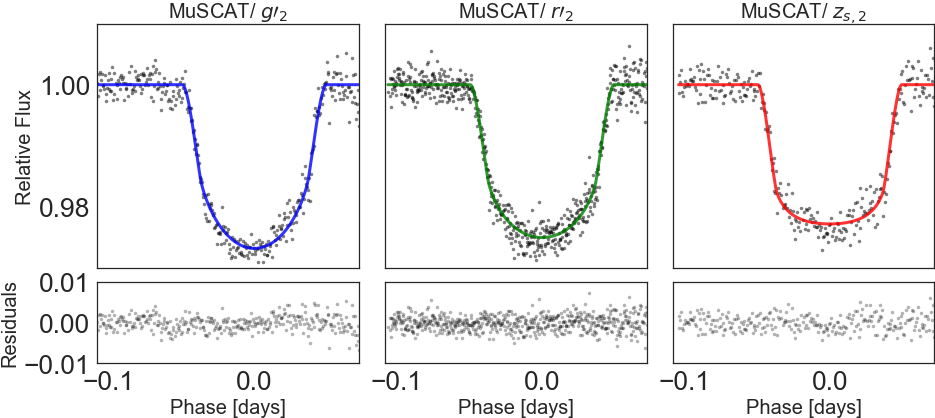
\includegraphics[width=1\columnwidth]{hatp12/grz_with_rms.png}
    \caption{Systematics-corrected transit light curves for HAT-P-44b (black dots) and best-fit transit models. %The binned flux data for $g'$, $r'$, and $z_s$-bands are shown by the blue, green, and red squares, respectively. 
    The blue, green, and red lines indicate the best-fit transit models for $g'$, $r'$, and $z_s$-bands. The lower panels show the residuals which have rms of 0.17\%,0.17\%,and 0.19\% for $g'$, $r'$, and $z_s$-bands respectively.}
\label{fig:hatp12_grz_multi}
\end{figure}

\begin{figure}
	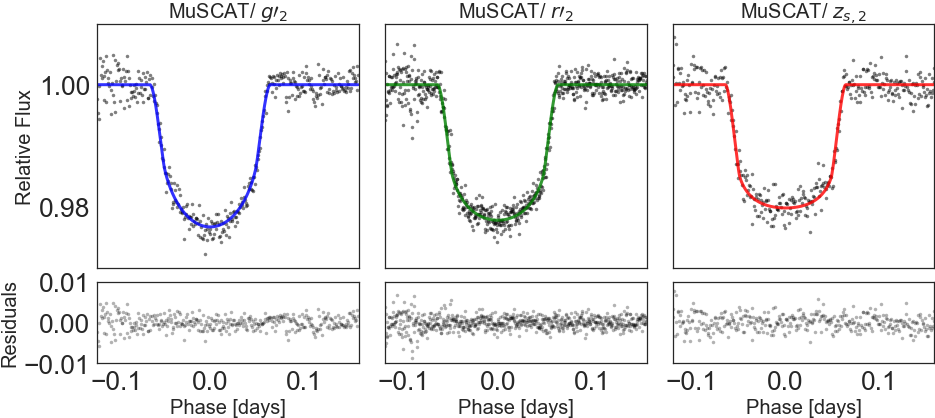
\includegraphics[width=1\columnwidth]{hatp44/grz_with_rms.png}
    \caption{Same as Fig.~\ref{fig:hatp12_grz_multi} but for HAT-P-12b. The lower panels show the residuals which have rms of 0.08\%,0.11\%,and 0.11\% for $g'$, $r'$, and $z_s$-bands respectively. %How about for n-minute bins?
    }\label{fig:hatp44_grz_multi}
\end{figure}

\begin{figure}
	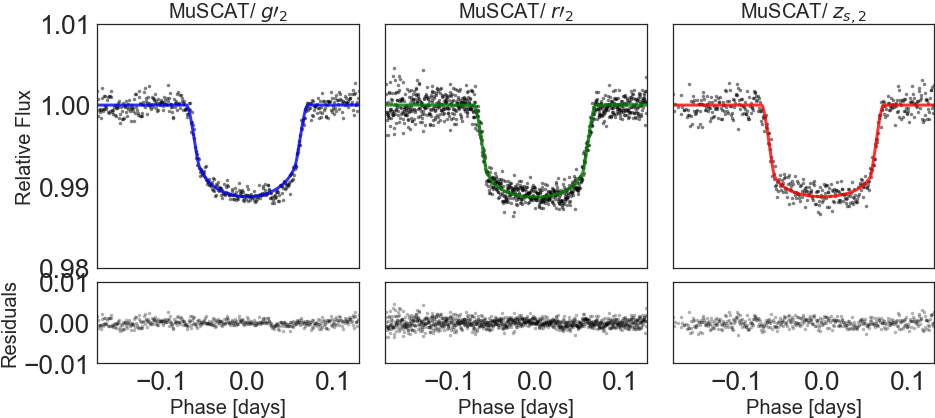
\includegraphics[width=1\columnwidth]{wasp21/grz_with_rms.png}
    \caption{Same as Fig.~\ref{fig:hatp44_grz_multi} but for WASP-21b. The lower panels show the residuals which have rms of 0.20\%,0.20\%,and 0.22\% for $g'$, $r'$, and $z_s$-bands respectively. %How about for n-minute bins?
    }\label{fig:wasp21_grz_multi}
\end{figure}

%Our results are in general agreement with those obtained by Hartman et al. (2009), Lee et al. (2012), and Sada et al. (2012).
%However, the recent analysis of a near-IR transmission spectrum from Hubble Space Telescope data by Line et al. (2013) yields a planet-to-star radius ratio that is ∼2.5\% smaller than the others

\paragraph{HAT-P-44b}
%See O-C diagram here
%http://var2.astro.cz/ETD/etd.php?STARNAME=HAT-P-44&PLANET=b
%HAT-P-44b since only single observation has been conducted towards this system. 
Assuming stellar radius in R$_s$= 0.95 $\pm$ 0.08 R$_{\odot}$ in Table~\ref{tab:params}, the measured mean planet radius is 1.228$\pm$ 0.015 R$_J$ compared to the published 1.242$\pm$ 0.106 R$_J$, a difference of $\sim$1.1\% which is well within the published uncertainty. Propagating the uncertainty in stellar radius however, we see that the uncertainty in R$_p$ cannot be any less than 0.7 R$_J$.

For impact parameter, we get $b$=0.16 $\pm$ 0.13 compared to the published 0.172$\pm$0.079, a difference of $\sim$ 9.5\%. Like HAT-P-12b, the large uncertainty in $b$ is reflected from the wide posterior in Fig.~\ref{fig:hatp44_tab}. For scaled semi-major axis, a/Rs=12.0440$\pm$0.0094 compared to the published 11.49$^{+0.46}_{-0.85}$, a difference of $\sim$4.8\% with smaller uncertainty. Therefore, $b$ and a$_s$ agree well with values found by \cite{Hartmann2014}. Moreover, the mean stellar density, $\rho_s$, is 1.84$_{-0.05}^{+0.03}$, which is consistent with the average density of 1.55$\pm$0.36 g/cm$^3$ solely determined from published mass and radius.

The full joint posterior distributions of transit center, $t_c$, impact parameter, $b$, and scaled semi-major axis, a$_s$ are shown in Fig~\ref{fig:hatp44_tab}. $t_c$, $b$, and a$_s$ agree well with values found by \cite{Hartmann2014}. Summary plots of other transit parameters shown in Fig.~\ref{fig:hatp44_q1q2}.

\begin{figure}
\centering
	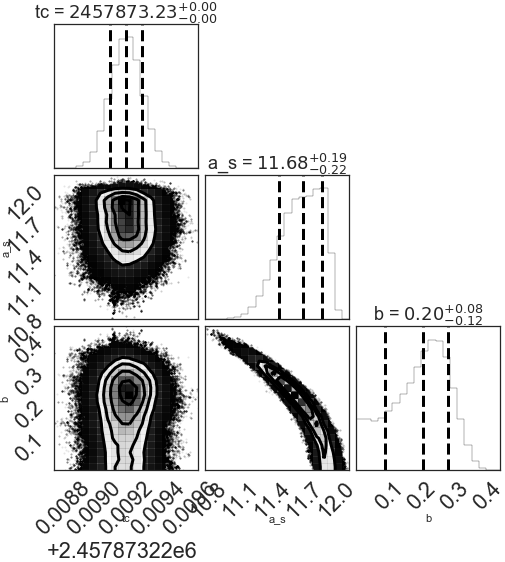
\includegraphics[width=8cm]{hatp12/joint_tc_a_b.png}
    \caption{Joint posterior probability distributions for transit center $t_c$ (columns 1), scaled semi-major axis, a$_s$ (columns 2), and impact parameter, $b$ (columns 3), from which the maximum $a \; posteriori$ (aka "best-fit" values) are computed. The plots on the diagonal are the marginalized posterior distribution where the vertical lines correspond to the adapted MAP and 1-$\sigma$ uncertainties.
    }
\label{fig:hatp12_tab}
\end{figure}

\begin{figure}
\centering
	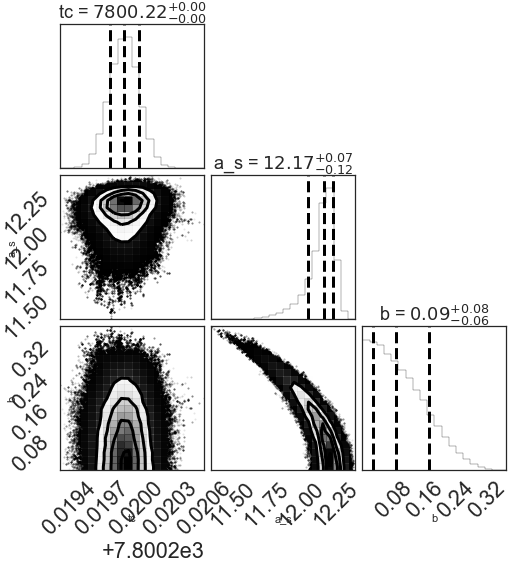
\includegraphics[width=8cm]{hatp44/joint_tc_a_b.png}
	\caption{Same as in Fig.~\ref{fig:hatp12_tab} but for HAT-P-44b.}
\label{fig:hatp44_tab}
\end{figure}

\begin{figure}
\centering
	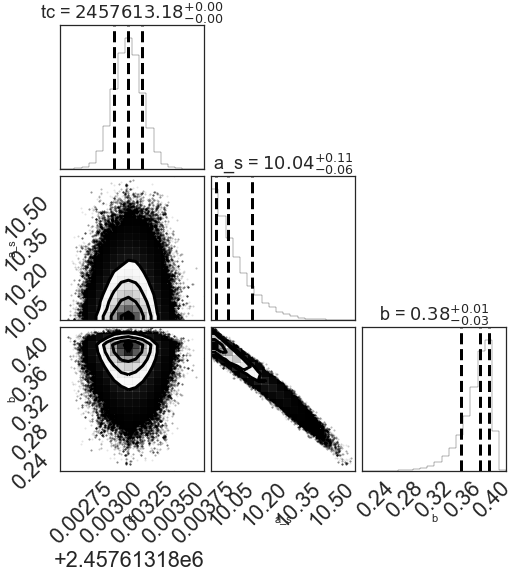
\includegraphics[width=8cm]{wasp21/joint_tc_a_b.png}
    \caption{Same as in Fig.~\ref{fig:hatp12_tab} but for WASP-21b.}
\label{fig:wasp21_tab}
\end{figure}

%------------------------------------------------------------------------
\paragraph{WASP-21b}
%See O-C diagram here
%http://var2.astro.cz/ETD/etd.php?STARNAME=WASP-21&PLANET=b

Assuming stellar radius in R$_s$= 1.136 $\pm$ 0.051 R$_{\odot}$ in Table~\ref{tab:params}, the measured mean planet radius is 1.097 $\pm$ 0.0044 R$_J$ compared to the published 1.07$\pm$ 0.06 R$_J$,
a difference of $\sim$2.5\%. %which is well within the published uncertainty. 
Therefore, we rule out the larger radius R$_p=$1.263$\pm$0.090 found by \cite{Southworth2012} including the fact that it reported larger uncertainties in R$_s$.
In any case, propagating the uncertainty in stellar radius however, we see that the uncertainty in R$_p$ cannot be any less than 0.55 R$_J$.

For impact parameter, we get $b$=0.3673 $\pm$ 0.0089 compared to the published 0.23$\pm$0.015, a difference of $\sim$ 60\% but still within the published uncertainty. Unlike our results for HAT-P-12b and HAT-P-44b, WASP-21b has smaller uncertainties in $b$ as reflected from the narrow posterior in Fig.~\ref{fig:wasp21_tab}. For scaled semi-major axis, a/Rs=10.10$\pm$0.12 compared to the published 9.62$\pm$0.17, a difference of $\sim$4.9\% with smaller uncertainty. Therefore, $b$ and a$_s$ agree well with values found by \cite{Bouchy2010}. Moreover, the mean stellar density, $\rho_s$, is 1.023$_{-0.018}^{+0.032}$, which is consistent with the average density of 0.855$\pm$0.068 g/cm$^3$.

The full joint posterior distributions of transit center, $t_c$, impact parameter, $b$, and scaled semi-major axis, a$_s$ are shown in Fig~\ref{fig:wasp21_tab}. Summary plots of other transit parameters shown in Fig.~\ref{fig:wasp21_q1q2}.


\begin{comment}
#measured Rp/Rs
g-band:	0.13182	$^{-0.00102}_{+0.00133}$
r-band:	0.13294	$^{-0.00157}_{+0.00018}$
z-band:	0.13109	$^{-0.00179}_{+0.00092}$

#measured Rp/Rs
g-band:	0.14196	$^{-0.00404}_{+0.00058}$
r-band:	0.14024	$^{-0.00150}_{+0.00092}$
z-band:	0.14025	$^{-0.00481}_{+0.00114}$

#measured Rp/Rs
g-band:	0.09670	$^{-0.00040}_{+0.00155}$
r-band:	0.09889	$^{-0.00039}_{+0.00059}$
z-band:	0.09998	$^{-0.00043}_{+0.00092}$
\end{comment}


%The uncertainty of individual parameters introduced by non-Gaussian correlations with other parameters is accounted for in a straightforward way by marginalizing the joint posterior over all remaining parameters (\cite{Benneke2012}). 

%in the JWST era
% ephemeris 
%lower uncertainties in:
% orbital period of 4.3012 d 
% mass of 0.35 M$_J$ and 
% radius of 1.24 R$_J$

%------------------------------------------------------------------------
\section{Improved Transit Ephemeris}
% Transit timing became one of the standard techniques in the analysis of transit observations. Commonly the mid-time of each transit observation is plotted into an observed minus calculated (O-C) diagram (Ford \& Holman 2007), where the difference between the observed transit mid-time and the mid-time obtained using the initial ephemeris is shown versus the observing epoch. In such a diagram, a non-zero slope indicate a varying orbital period, while e.g. periodic deviations from a linear trend indicate perturbing forces. %Transit intervals indicating deviations from a strictly Keplerian motion and thus yet hidden planets in the observed system.

The addition of even a single follow-up transit measurement can improve the ephemeris of the planet especially in the case of HAT-P-44b which was observed only a few epochs as reported in the discovery paper. For each planet we analyze in this work, we compute updated ephemerides using the mid-transit times from our work reported in Table~\ref{tab:hatp12_map}--\ref{tab:wasp21_map} and $T_0$ from the discovery paper: % of the previous observations:
\begin{equation}
T_c(BJD_{TDB})=T_0+E \times P
\end{equation}
where $E$ is the epoch and $P$ is the orbital period. 

\paragraph{HAT-P-44b}
To check if our result is consistent with other observation, we enlarged the sample by considering mid-transit times available in the literature or on websites such as the Exoplanet Transit Database (ETD)\footnote{http://var2.astro.cz/ETD/} %TRansiting ExoplanetS and CAndidates (TRESCA) archive, 
which essentially contain light curves obtained by amateur astronomers. We selected only the light curves with a data quality index higher than 3. %(see Table~\ref{tab:hatp44_ephem}). 
By fitting these data with a linear function, we derive the improved transit ephemeris as
\begin{equation}
T_c(\rm{BJD_{TDB}})= 2457800.21961500+4.30119154 \times E
\end{equation}
where $E$ is the relative transit epoch and the number in parentheses on the right represents the last two digits of 1$\sigma$ uncertainty. %The residuals from this ephemeris, $\Delta T_c$, are appended to Table~\ref{tab:hatp44_ephem} and shown in Figure~\ref{fig:hatp44_ephem}.
 
%bivariate correlated errors and intrinsic scatter 

\begin{comment}
\begin{table}
\centering
\label{tab:hatp44_ephem}
\caption{A comparison between the results obtained in our analysis and the literature data for the measured Transit Timing ($Tc$), Timing Residual from the Linear Ephemeris ($T_c$), and Impact Parameter ($b$) for each transit of HAT-P-44b}
\begin{tabular}{lllll}
Transit epoch & Telescope & $T_c$ (BJD$_{TDB}$-2450000) & $\Delta T_c$ (days) & $b$ \\
\hline
0 & OAO188 & 7800.219893$^{0.00013}_{-0.00013}$ &  & \\
\hline
\end{tabular}
\end{table}
\end{comment}

\paragraph{HAT-P-12b}
%https://exoplanetarchive.ipac.caltech.edu/cgi-bin/DisplayOverview/nph-DisplayOverview?objname=HAT-P-12+b&type=CONFIRMED_PLANET
For HAT-P-12b, we derive the improved transit ephemeris as
\begin{equation}
T_c(\rm{BJD_{TDB}})= 2454419.19570000+3.21604609 \times E
\end{equation}
where $E$ is the relative transit epoch and the number in parentheses on the right represents the last two digits of 1$\sigma$ uncertainty.
The residuals from this ephemeris %, $\Delta T_c$, are appended to Table~\ref{tab:hatp12_ephem} and 
is shown in Figure~\ref{fig:hatp12_ephem}.

\begin{comment}
\begin{table}
\centering
\label{tab:hatp12_ephem}
\caption{Same as Table~\ref{tab:hatp44_ephem} but for HAT-P-12b.}
\begin{tabular}{lllll}
Transit epoch & Telescope & $T_c$ (BJD$_{TDB}$-2450000) & $\Delta T_c$ (days) & $b$ \\
\hline
X & FLWO 1.2m & 4419.19556$\pm$0.00020 &  & - \\ %Sada&Ramon-Fox+2016
X & UdMO 0.36m &4419.19584$\pm$0.00009 & & 0.211$^{+0.066}_{-0.078}$ \\ %Hartmann+2009
0 & OAO 1.88m & 7873.2292$\pm$0.0001 &  & 0.211$\pm$0.1402 \\ 
\hline
\end{tabular} 
\end{table}
\end{comment}

\begin{comment}
%2454419.19584±0.00009 (Sada & Ramón-Fox 2016)
%2454419.19556±0.00020 (Hartmann 2009)
%2457613.1832 ± (this study)
%See O-C diagram here
%http://var2.astro.cz/ETD/etd.php?STARNAME=HAT-P-12&PLANET=b
\end{comment}

\paragraph{WASP-21b}
%https://exoplanetarchive.ipac.caltech.edu/cgi-bin/DisplayOverview/nph-DisplayOverview?objname=WASP-21+b&type=CONFIRMED_PLANET
For WASP-21b, we derive the improved transit ephemeris as
\begin{equation}
T_c(\rm{BJD_{TDB}})= 2454743.03822454+4.32251406 \times E
%2454743.04632158+4.32250054xE (with other data)
\end{equation}
%where $E$ is the relative transit epoch and the number in parentheses on the right represents the last two digits of 1$\sigma$ uncertainty.
%Ciceri+2013: T0(BJD_TDB) = 2 454 743.04054 (71)+ 
%                 4.322 5186(30) E
%Seelinger+2015:  4.322 51(22)
%Bouchy+2010:     4.322 4(24)  # −0.000 019
%Barros+2011:     4.322 50(31)
%Southworth+2012: 4.322 50(31)

The residuals from this ephemeris%, $\Delta T_c$, are appended to Table~\ref{tab:wasp21_ephem} and
is shown in Figure~\ref{fig:wasp21_ephem}.
%Selinger+2015: A new ephemeris is determined for the system, i.e. T0= 245 5084.519 74 ± 0.000 20 (HJD) and P= 4.322 5060 ± 0.000 0031 d. 
%In addition, the results of the analysis of two transit events of Ciceri et al. (2013) and one transit observation of Southworth (2012) are also taken into account. Concerning the O-C diagram, we found that a period change of (2.63 ± 0.17) s removes the linear trend which is present in the data fitted with the initial ephemeris. 

\begin{comment}
Seelinger+2015
However, regarding inclination and reverse fractional stellar radius
we do see a significant difference between our results and the
initial values published by Bouchy et al. (2010). This was also found
by other authors before. As discussed in Barros et al. (2011), this
result is a consequence of the assumption of Bouchy et al. (2010)
that the planet host star is a main-sequence star, while Barros et al.
(2011) found that the star starts evolving off the main sequence and
thus its radius increases. This in turn leads to corrections of the
stellar and hence planetary properties.

\begin{table}
\centering
\label{tab:wasp21_ephem}
\caption{Same as Table~\ref{tab:hatp44_ephem} but for WASP-21b.}
\begin{tabular}{lllll}
Transit epoch & Telescope & $T_c$ (BJD$_{TDB}$-2450000) & $\Delta T_c$ (days) & $b$ \\
\hline
X & YETI      & 4743.04217$\pm$0.00065 & & - \\ %Seelinger+2011
X & FLWO 1.2m & 4743.0419$^{+0.0019}_{-0.0022}$&  & 0.23$^{+0.12}_{-0.15}$ \\ %Bouchy+2010
0 & OAO 1.88m & 7873.2292$\pm$0.001 & & 0.2299$\pm$0.1404 \\
\hline
\end{tabular}
\end{table}
\end{comment}

\section{Transit Timing Variation and Transit Duration Variation}
The central times of the transits are also useful to check for the presence of additional bodies. If another planetary object is a member of the system, it should gravitationally interact with the known planet, causing a periodical variation in $T_0$. Other
phenomena can cause timing variations, for example starspots. %(\cite{Barros2013})
We plot the residuals of the linear fits to the times of minimum light below. In both cases we do not find any clear evidence of periodic variations in the transit timings.

\begin{figure}
\centering
	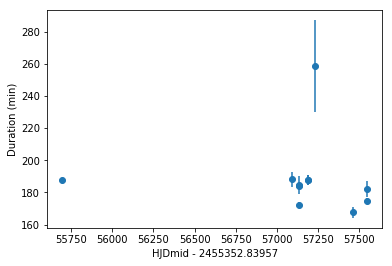
\includegraphics[width=7cm]{hatp44/tdv.png}
    \caption{Updated O-C diagram of HAT-P-44b.}
\label{fig:hatp44_tdv}
\end{figure}

\begin{figure}
\centering
	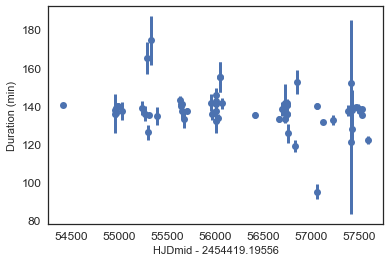
\includegraphics[width=7cm]{hatp12/tdv.png}
    %\caption{Transit duration variation of HAT-P-12b.}
    \caption{Updated O-C diagram of HAT-P-12b. %The transit midpoint at various epochs can be fit with a linear ephemeris.
    }
\label{fig:hatp12_tdv}
\end{figure}
\begin{figure}
\centering
	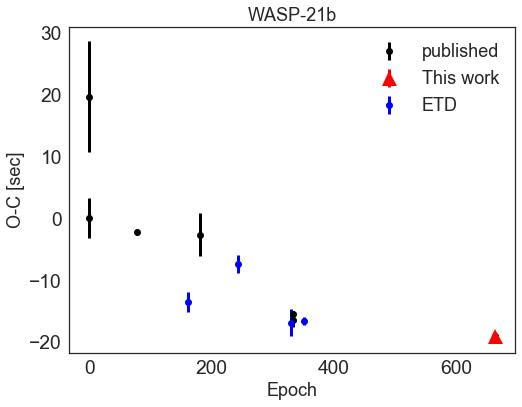
\includegraphics[width=7cm]{wasp21/wasp21_tdv.png}
    \caption{Updated O-C diagram of WASP-21b. %The transit midpoint at various epochs can be fit with a linear ephemeris.
    }
\label{fig:hatp12_oc}
\end{figure}

\begin{comment}
\begin{table}
\centering
\caption{}
\begin{tabular}{lllllll}
& $T_c$ - 2450000 & a/Rs & Rp/Rs & i \\
\hline
Bouchy et al. (2010) &4743.0426 ± 0.0022 & 6.05$^{+0.03}_{−0.04}$ &0.1040$^{+0.0017}_{−0.0018}$ &88.75 $^{+0.70}_{−0.84}$ \\
Barros et al. (2011a) &5084.52048 ± 0.00020 & 9.68 $^{+0.30}_{−0.19}$ &0.1071$^{+0.0009}_{−0.0008}$ & 87.34 ± 0.29 \\
Southworth (2012) &5084.52040 ± 0.00016 &9.35 ± 0.34 &0.1095 ± 0.0013 &86.77 ± 0.45 \\
Ciceri et al. (2013) &4743.04054 ± 0.00071 &9.46 ± 0.27 &0.1055 ± 0.0023 & 86.97 ± 0.33 \\
Seelinger et al. (2015) &4743.04217 ± 0.00065 &9.62 ± 0.17 &0.1030 ± 0.0008 &87.12 ± 0.24 \\
This work & 7613.1832 & 10.0979 & 0.1000 ± 0.005 & \\
\hline
\end{tabular}
\end{table}
\end{comment}

\begin{comment}
The residuals from this ephemeris, $\Delta T_c$, are appended to Table 5 and shown in Figure 4. The $\chi^2$ value of the linear fit is 15.5 for five degrees of freedom (DOF), meaning that the linear function nominally has a 2.6 $\sigma$ discrepancy with the observed data. However, discrepancies with similar levels often arise in ground-based T_c observations, possibly due to unknown systematics rather than the true timing variations. Therefore, we do not consider it to be a noticeable TTV signal at this point. We note that the $T_c$ value of the transit observed by Nascimbeni et al. (2011) departs from our new ephemeris by 2.8$\sigma$, causing a systematic shift in their ephemeris (gray dashed line in Figure 4), which has propagated to be $\sim$ 15 minutes at the time of our observation. In any case, the correction of the ephemeris in this work should be useful for future observations.

Next we search for TDVs to check for any evidence of
additional bodies. The transit duration is generally expressed as
the time interval between the first and fourth contacts of a
transit, T 14 , which is a function of a R s , b, and R p R s . We here assume that a R s and R p R s do not vary with time within the
uncertainties and search for the time dependence of b instead of
T 14 . The measured b values of the seven transits and their
uncertainties are listed in Table 5 and shown in Figure 5. A
constant fit to these values gives the mean of b = 0.9015±0.0024 with c 2 = 7.5 for dof = 6, meaning that no significant variation is observed.

To demonstrate the increased observing efficiency afforded by our MuSCAT observations, we compute the propagated timing uncertainty in %in mid-2019
\begin{equation}
\sigma(t_c)=\sqrt{\sigma(t_0)^2+(n\sigma (P))^2}
\end{equation}
where $\sigma (t_c)$ is the propagated timing uncertainty, $\sigma(t_0)$ is the uncertainty in the starting transit center, $n$ is the number of orbits into the future for which to compute the propagated uncertainty, and $\sigma (P)$ is the uncertainty in the orbital period. 
\end{comment}

We note that the transit midpoint at various epochs can be fit with a linear ephemeris for all planets, consistent with previous results.

\section{Transit Depth Variation}\label{sec:spectrum}
%Caveat
%Stellar variability, in the form of star spots and faculae, can affect the measured transit depth of an exoplanet and hence its spectrum and retrieved physical properties (Pont et al. 2008; Silva Valio 2008; Czesla et al. 2009; Wolter et al. 2009; Agol et al. 2010; Berta et al. 2011; Carter et al. 2011; Desert et al. 2011; Sing et al. 2011; Fraine et al. 2014; McCullough et al. 2014; Oshagh et al. 2014; Damasso et al. 2015; Barstow et al. 2015; Zellem et al. 2015; Rackham et al. 2017). As a worst case scenario for very active stars, unocculted spots can cause an underestimation of the planet-to-star radius ratio of up to 4% at near-infrared wavelengths and 10% at visible wavelengths while faculae can cause an overestimation of the planet-to-star radius ratio of up to ∼0.2% at near- infrared wavelengths at ∼3% at visible wavelengths (Oshagh et al. 2014). Unocculted spots can also mimic a Rayleigh scattering slope indicative of haze; for example, the visible and near-IR slope of the exoplanet HD 189733b’s transit absorption spectrum, interpreted as Rayleigh scattering by haze particles (Pont et al. 2008, 2013; Sing et al. 2011, 2016), has also been interpreted as unocculted star spots on its active K0 host star (McCullough et al. 2014). Unocculted spots can also introduce false molecular spectral modulation into an exoplanet’s spectrum, such as H2O if the spots are sufficiently cool (Fraine et al. 2014; Barstow et al. 2015). Stellar faculae, which are brighter than the stellar photosphere, decrease the transit depth at optical wavelengths (Rackham et al. 2017). Evolving unocculted spots on an active host star could also pose a problem when stitching data together from multiple epochs spanning multiple wavelengths, as will be required to completely sample an exoplanet from 0.6–28 µmwith NASA’s JamesWebb Space Telescope (JWST; Barstow et al. 2015). Therefore spectroscopic observations of an exoplanet orbiting an active star have the potential to result in an erroneous interpretation of its atmospheric properties, if the measurements have sufficient precision. As transit spectroscopic measurements become increasingly precise, especially in the JWST era, the possibility of contamination of the transit signal by star spots must be examined with care.
We plotted the posterior distributions of Rp/Rs of each band in the first column of Fig.~\ref{fig:hatp44_RpRs}--\ref{fig:wasp21_RpRs}; in the second column, we superpose the systematic-corrected data and best fit transit models of each band on top of each other to illustrate the relative transit depth variation in each band. In all cases, we achieved the smallest uncertainty (i.e. narrow distribution) in r-band.%In the case of WASP-21b, the relative spread of each distribution in Fig.~\ref{fig:wasp21_RpRs} (a) is not apparent in Fig.~\ref{fig:wasp21_RpRs} (b).  

\begin{comment}
To calculate the flux of the model spectrum as if it goes through the MuSCAT filter,
\begin{equation}
\frac{\int{E_f F_p \times d\lambda}}{\int{E_f d\lambda}}
\end{equation} 
where $E_f$ is the filter transmission, $F_p$ is the flux of model spectrum at the particular wavelength $\lambda$.
\end{comment}

%-----------------------------------------------------------

\begin{figure}
\centering
\begin{subfigure}{.5\textwidth}
	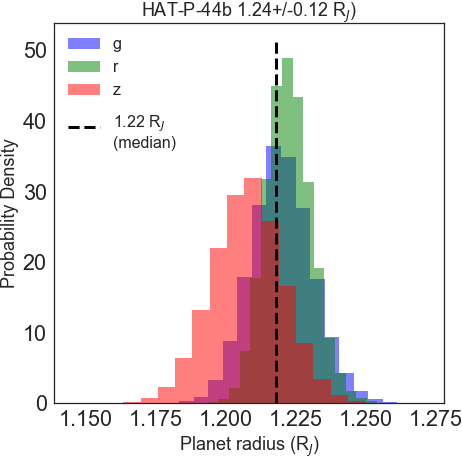
\includegraphics[width=6cm]{hatp44/radius_ratios_Rjup.png}
    \caption{Posterior distributions of Rp/Rs in each band.}
\end{subfigure}%
\begin{subfigure}{.5\textwidth}
	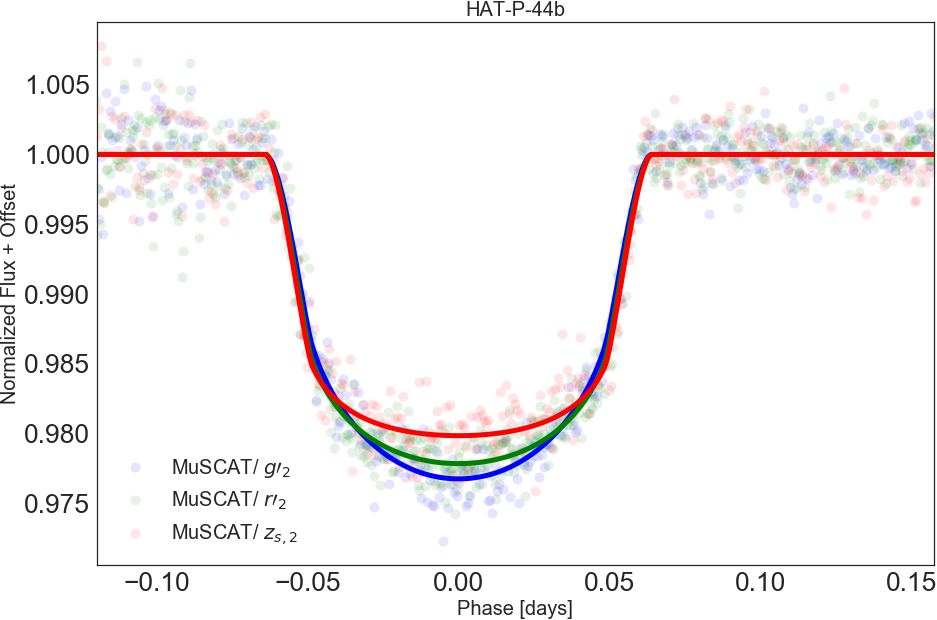
\includegraphics[width=8cm]{hatp44/grz_multi_stacked.png}
    \caption{Superposed data and best fit transit model}
    \label{fig:hatp44_stacked}
\end{subfigure}
\caption{(a) Maximum a posteriori (MAP) value of Rp/Rs in each band shows that their difference is marginal; (b) The best fit transit model (colored lines) and systematics-corrected data (colored points) are stacked compare transit depth variation.}
\label{fig:hatp44_RpRs}
\end{figure}

\begin{figure}
\centering
\begin{subfigure}{.5\textwidth}
	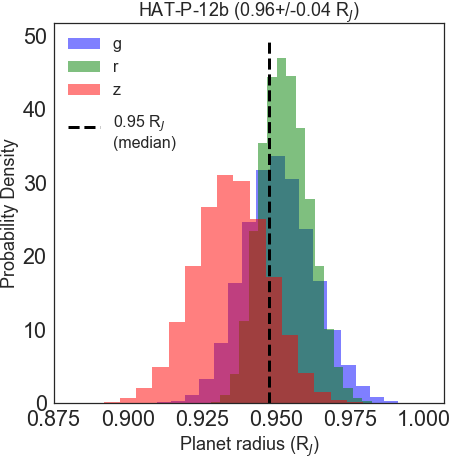
\includegraphics[width=6cm]{hatp12/radius_ratios_Rjup.png}
    \caption{Posterior distributions of Rp/Rs in each band.}
\end{subfigure}%
\begin{subfigure}{.5\textwidth}
	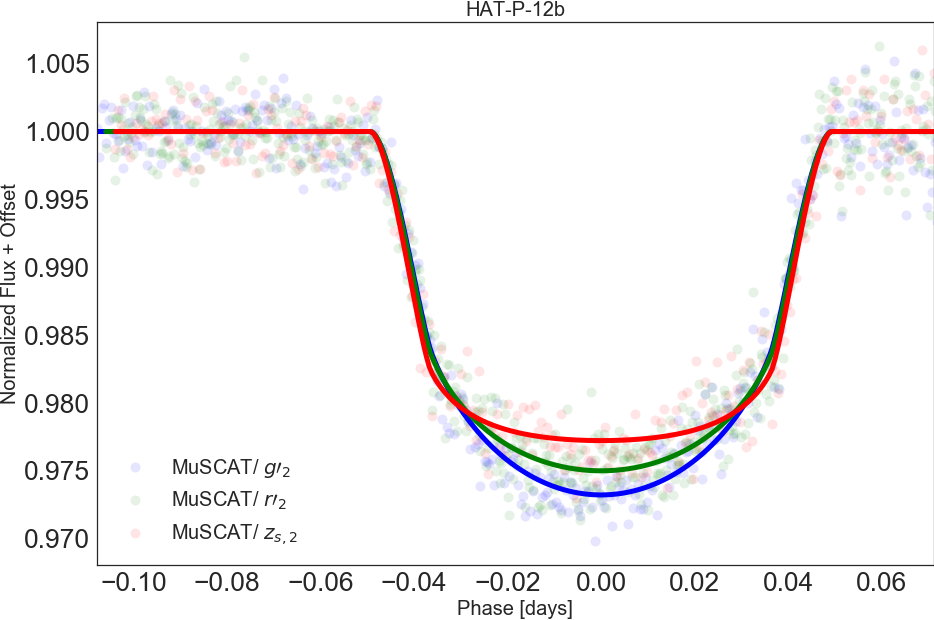
\includegraphics[width=8cm]{hatp12/grz_multi_stacked.png}
    \caption{Superposed data and best fit transit model.}
    \label{fig:hatp12_stacked}
\end{subfigure}
\caption{Same as Fig~\ref{fig:hatp44_RpRs} but for HAT-P-12b. Detection of Rp/Rs variation is also marginal.}
\label{fig:hatp12_RpRs}
\end{figure}

\begin{figure}
\centering
\begin{subfigure}{.5\textwidth}
	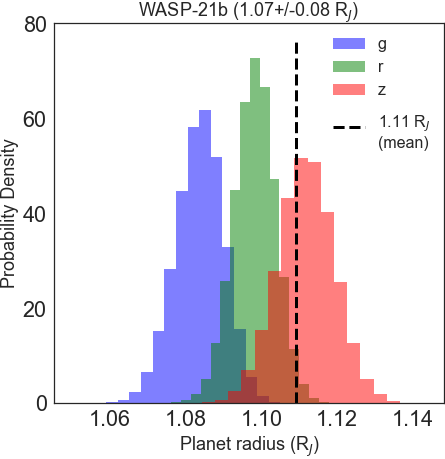
\includegraphics[width=6cm]{wasp21/radius_ratios_Rjup.png}
    \caption{Posterior distributions of Rp/Rs in each band.}
\end{subfigure}%
\begin{subfigure}{.5\textwidth}
	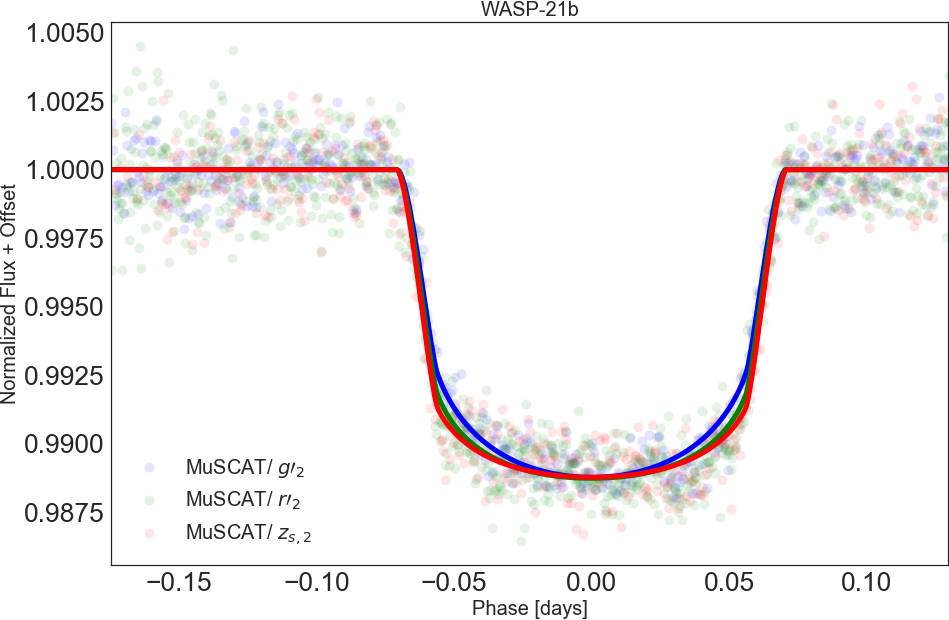
\includegraphics[width=8cm]{wasp21/grz_multi_stacked.png}
    \caption{Superposed data and best fit transit model.}
    \label{fig:wasp21_stacked}
\end{subfigure}
\caption{Same as Fig~\ref{fig:wasp21_RpRs} but for WASP-21b. Detection of Rp/Rs variation is marginal (2.8$\sigma$) and the trend is not of atmospheric origin and instead such feature is best explained by an unocculted spot on the surface of WASP-21 (see text for details).}
\label{fig:wasp21_RpRs}
\end{figure}

%------------------------------------------------------------------------
\paragraph{Empirical Scale height and Mean molecular weight}
\cite{Benneke2012} derived an equation used to estimate the scale height $H$ given Rp/Rs measurements:
\begin{equation}
\label{eq:H_emp}
H \approx \frac{R_{P,\lambda_2}-R_{P,\lambda_1}}{4 \ln \Big(\frac{\lambda_1}{\lambda_2}\Big)}
\end{equation}
given two transit depth observations at $\lambda_1 \& \lambda_2$ in the Rayleigh scattering regime. 
%show for general atmospheres that the value of the mean molecular mass can be determined by measuring the slope of the Rayleigh scattering signature at short wavelengths, dRP,λ d(lnσλ) , with which the ”observed” planet radius, RP,λ, changes as a function of the extinction cross section, σλ, across different wavelengths.

\cite{Benneke2012} also showed that the mean molecular mass $\mu$ of a general atmosphere can be estimated via
\begin{equation}
\label{eq:mu}
\mu =\frac{4k_BT}{gR_*}\frac{\ln \Big(\frac{\lambda_1}{\lambda_2}\Big)}{\Big(\frac{R_P}{R_*}\Big)_{\lambda_2} -\Big(\frac{R_P}{R_*}\Big)_{\lambda_1}} \times \Big(1\pm\frac{\delta T}{T}\Big)
\end{equation}
where $T$ is the atmospheric temperature. The factor $(1\pm \frac{\delta T}{T})$ accounts for the inherent uncertainty due to the uncertainty, $\delta T$, at the observed planet radius $r = R_{P,\lambda}$. % the mean molecular mass varies by a factor on the order of 8−20 between hydrogen-dominated atmospheres and atmospheres mainly composed of H$_2$O, N$_2$, or CO$_2$.

Table~\ref{tab:mu} summarizes our results for empirical $H$ and $\mu$ using Eq.~\ref{eq:mu} and Eq.~\ref{eq:mu} where we assumed $T\approx T_{eq}$. We used r-band as reference wavelength because of smaller uncertainty. These estimates are only valid for Rayleigh scattering regime. As apparent in Fig.~\ref{fig:wasp21_RpRs}, WASP-21b spectrum does not show apparent Rayleigh slope and hence no estimates are provided in Table~\ref{tab:mu}. For HAT-P-12b, the empirical scale height estimate ($\sim$700 km) at the empirical $\mu$=2.92 amu from the theoretical value ($\sim$500 km) by a large margin. 

%This is 
\begin{table}
\centering
\caption{Empirical estimates of scale height and mean molecular weight of the planet's atmosphere based on Rp/Rs measurements.}
\label{tab:mu}
\begin{tabular}{llllll} 
\hline
          &\multicolumn{2}{c}{$H$ (km)}& $\mu$ (amu) \\ %g (m/s$^2$) & $T_{eq}$ (K) &
          &  theoretical & empirical & & \\
\hline
HAT-P-12b & 615.6 & 765.6 & 2.88$\pm$0.5 \\ % 5.62 $\pm$ 0.01 &  963$\pm$16  &
HAT-P-44b & 708.2 & 613.6 & 5.79$\pm$0.8 \\ %& 5.62 $\pm$ 0.01 & 1108$^{+51}_{-32}$ 
WASP-21b  & 950.0 & -- &-- \\ %5.07 $\pm$ 0.035 & 1340$\pm$32   &
\hline
\end{tabular}
\end{table}

%Teq for a planet around HAT-P-14, HAT-P-11, and GJ1214 is calculated to be 1652 K, 861 K, and 398 K, respectively.
%We note that $T_{eq}$ can vary by up to $\sim15\%$ in the range of 2 < P(days) < 5 and 0 < $A$ < 0.7; however, the impact of this change on $H$ is trivial compared with that of the possible range of the surface gravity $g_p$, which extends by a factor of several or even two orders of magnitude depending on the planetary size.

%------------------------------------------------------------------------

%=======================================================================
\section{Atmospheric Models}
%Spectrum modeling is done by fitting the data with a synthetic spectrum created using best estimates of the desired atmospheric properties %(using prior knowledge and new observations), 
%such as the mixing ratios of the molecular constituents and the surface/cloud-top pressure.
We plotted the measured Rp/Rs with uncertainties as a function of wavelength (i.e. transmission spectrum) in Fig.~\ref{fig:atm_hatp44b}--\ref{fig:atm_wasp21b}. The vertical error bars correspond to measurement error and horizontal error bar correspond to the width of the bandpass of MuSCAT filters.
%The calculated model spectrum is shown as black solid line in Figure 6 where the initial model is vertically shifted such that the mean value of the model fits to the observation. Again, the expected Rp/Rs variations of this planet are too low with respect to the observational uncertainties.
In addition, to compare the observed data with a theoretical atmospheric model, we calculate a model spectrum of Rp/Rs for each planet. Detailed discussion of spectrum modeling procedure is beyond the scope of this thesis. The model description and procedure are detailed in \cite{Kawashima2015} and \cite{Kawashima2017} (see also \cite{Fukui2014}) and so we summarize the relevant information as follows.
% sensitivity of transmission spectra to the production rate of haze monomers, which relates to the amount of UV irradiation from the host star. 

%The calculation is done based on the method described in Fukui et al. (2014), but in this case line absorption of H 2 S, OCS, O 2 , TiO, and VO are taken into account in addition to those treated in Fukui et al. (2014) (H 2 , H 2 O, CH 4 , CO, CO 2 , NH 3 , N 2 , Na, and K). 
%Further, the absorption cross sections for these species are calculated on a wavelength-by-wavelength basis with a step size given by dividing the wavelength range from 0.3 to 1.0 $\mu$m by 2.5$\times$10 5 in log scale without taking the geometric mean for a  certain range of wavelengths as done in Fukui et al. (2014). An initial model spectrum is calculated by assuming that R0, the planetocentric distance at which the atmospheric pressure is 10 bar, is equal to 1.219 R Jup (Southworth 2012). 

%Theoretical Rayleigh Scattering Slope: Seager and Benneke (2012)
We calculated the spectrum models for 1 $\times$ Solar (case 1) and 100 $\times$ Solar metallicity clear atmospheres (case 2) for each exoplanet. For case 1, we consider an atmosphere with solar elemental abundances. This model atmosphere is composed of 11 elements, namely H, He, C, N, O, Na, K, P, S, Ti, and V with abundance ratios similar to those of the Solar system.% as shown in Table~\ref{tab:abundances}. 
The term metallicity means the total mass fraction of the nine elements other than H and He, with adapted value of 0.01036. For case 2, we consider a H-dominated atmosphere with metallicity enhanced by a factor of 100 relative to the solar metallicity (i.e. 1.036).
%The files without the name “smooth” is ones for the spectrum model of high resolution and ones with the name “smooth” are for the spectrum models smoothed for the clarity by averaging over the wavenumber range of 63.2 cm$^{-1}$ for each point. 
In both models, it is assumed that the atmospheres have thermochemical equilibrium compositions and isothermal structures with the equilibrium temperatures reported Table~\ref{tab:params}. %Note that MuSCAT filters do not overlap with emission lines by Na D doublet ($\sim$0.589 $\mu$m) and the potassium resonance doublet ($\sim$0.77 $\mu$m) as shown by the models.
Also, as pressure-radius relation is unknown for exoplanets, we found the appropriate value of radius at which the pressure is 10 bar that matches the theoretical spectrum with the transit radius we observed. The value of degrees of freedom (d.o.f.) is 2 for all the cases as there is 1 parameter, the value of radius at which the pressure is 10 bar. 

The data and model spectra are shown in Fig.~\ref{fig:atm_hatp12b}--\ref{fig:atm_wasp21b}. To discriminate which model is favored, the (reduced) $\chi^2$ %goodness of fit 
are computed and summarized in Table~\ref{tab:chi2}. Individual cases are discussed below.

\paragraph{HAT-P-12b}
As seen in Fig.~\ref{fig:atm_hatp12b}, the measured Rp/Rs coincide with either model because of the large uncertainties in Rp/Rs (hereby referred to as fractional uncertainties). %The measured Rp/Rs in all MuSCAT bands are consistent with the atmospheric model with $\chi^2$/dof=0.950, %$\chi^2$=28.0 and dof=2
%implying that our measured uncertainties in the individual band are underestimated. 
%Rp/Rs is not constant over the observed wavelength range within 1.8$\sigma$. 
%The larger value for (reduced) $\chi^2$ implies that the 100$\times$ Solar model is more favored.
The values of $\chi^2$ / d.o.f. are 0.217 and 0.711 for 1 $\times$ Solar and 100 $\times$ Solar atmospheres, respectively. Our photometric precision is not enough to distinguish between two models.
%We note that that our results for HAT-P-12b cannot conclusively distinguish between our two atmospheric models. 
%This is because the 1$\sigma$ uncertainties of the measured Rp/Rs is at the level of $\sim$2 times as large as one scale height (See Table~\ref{tab:H/u}). In the case of HST/STIS observations, $H/\sigma_{Rp/Rs}$ is between 0.5-2.2 scale heights in the optical wavelengths.
%can also be interpreted as consistent with a flat spectrum without the knowledge of the published HST/STIS spectra. 

\paragraph{HAT-P-44b}
%HAT-P-44b was observed by \cite{Hartmann2014} in the $r,i,I$-bands but their modeling assumed constant transit depth in all filters. 
Similar to HAT-P-12b, the measured Rp/Rs for each band coincide with either model spectrum as shown in Fig.~\ref{fig:atm_hatp44b} because of the large uncertainties. However, we achieve a smaller absolute individual fractional uncertainty, the largest among them has absolute amplitude of $\sim$0.006 for z-band. %The measured Rp/Rs in all MuSCAT bands are consistent with the atmospheric model with $\chi^2$/dof=0.950, %$\chi^2$=28.0 and dof=2
%implying that our measured uncertainties in the individual band are underestimated. 
%Rp/Rs is not constant over the observed wavelength range within 1.8$\sigma$. 
%The larger value for (reduced) $\chi^2$ implies that the 100$\times$ Solar model is more favored.
The values of $\chi^2$ / d.o.f. are 0.884 and 0.363 %0.406 and 0.151 
for 1 $\times$ Solar and 100 $\times$ Solar atmospheres, respectively. Our photometric precision is not enough to distinguish between two models.

\paragraph{WASP-21b}
Unlike HAT-P-12b and HAT-P-44b, the measured Rp/Rs do not coincide with either model spectrum except for the r-band with absolute amplitude of$\sim$0.002, as shown in Fig.~\ref{fig:atm_wasp21b}.
The values of $\chi^2$ / d.o.f. are 3.1 and 2.4 %8.00 and 4.40 
for 1 $\times$ Solar and 100 $\times$ Solar atmospheres, respectively, implying that both models cannot explain the data even with the small uncertainties. %As opposed to Rayleigh scattering feature (negative slope) in the optical wavelength, the apparent trend (positive slope) is inconsistent with our atmospheric model. We discuss the nature of this feature in \S \ref{sec:discussion}.

\begin{table}
\centering
\caption{$\chi^2$ value for both atmosphere models for each data set. The reduced $\chi^2$ is enclosed in parenthesis.}
\label{tab:chi2}
\begin{tabular}{llll}
& 1 $\times$ Solar & 100 $\times$ Solar \\
\hline
HAT-P-12b & 0.266 (0.515)  & 0.471 (0.687)  \\   
HAT-P-44b & 0.782 (0.884)  & 0.132 (0.363)  \\    
WASP-21b  & 9.978 (3.159)  & 5.660 (2.379)  \\       
%0.406)     &   (0.151)
%(8.00)  &  (4.40)
\hline
\end{tabular}
\end{table}

\begin{figure}
\centering
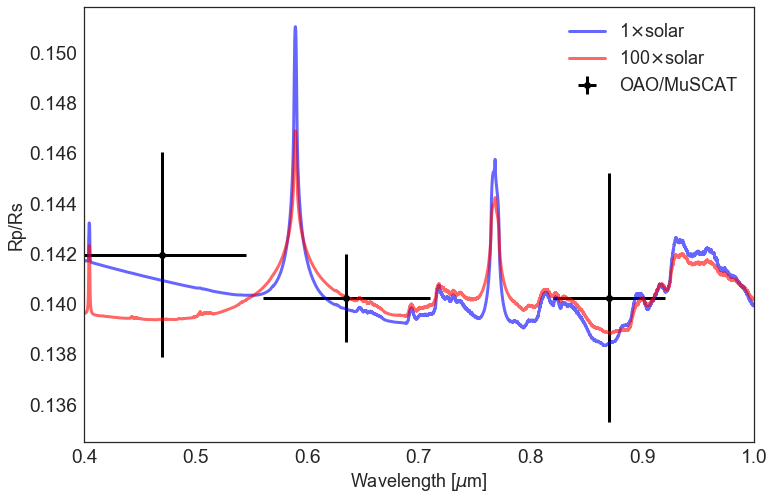
\includegraphics[width=12cm]{hatp12/atm_model.png}
\caption{HAT-P-12b transmission spectrum. From left to right, the three data points %black circle, square, and triangle 
correspond to MuSCAT g, r, and z-bands, respectively. The horizontal bars indicate the full width at half maximum of the response functions of the respective filter. Spectrum models with 1 $\times$ Solar (blue) and 100 $\times$ Solar atmospheres (green) assumes $T_{eq}$ = 963$\pm$16 K. 
 %The Rayleigh slope we observed are much steeper than the clear atmosphere models implying that haze or aerosol may exist in the atmosphere. 
 The values of $\chi^2$ / d.o.f. are 0.52 and 0.69 for 1 $\times$ Solar and 100 $\times$ Solar atmospheres, respectively, implying that our photometric precision is not enough to distinguish between two models.
 }
\label{fig:atm_hatp12b}
\end{figure}

\begin{figure}
\centering
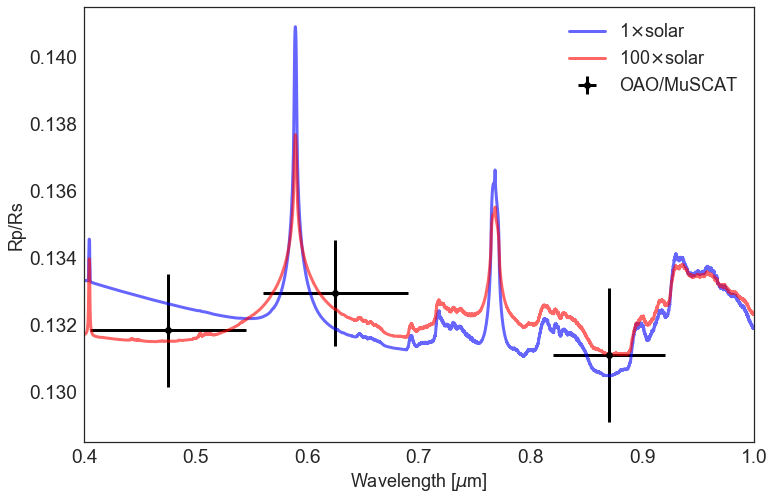
\includegraphics[width=12cm]{hatp44/atm_model.png}
\caption{Same as Fig~\ref{fig:atm_hatp12b} but for HAT-P-12b assuming $T_{eq}$ = 963$\pm$16 K. 
The values of $\chi^2$ / d.o.f. are 0.88 and 0.36 for 1 $\times$ Solar and 100 $\times$ Solar atmospheres, respectively, implying that our photometric precision is not enough to distinguish between two models.}
\label{fig:atm_hatp44b}
\end{figure}

\begin{figure}
\centering
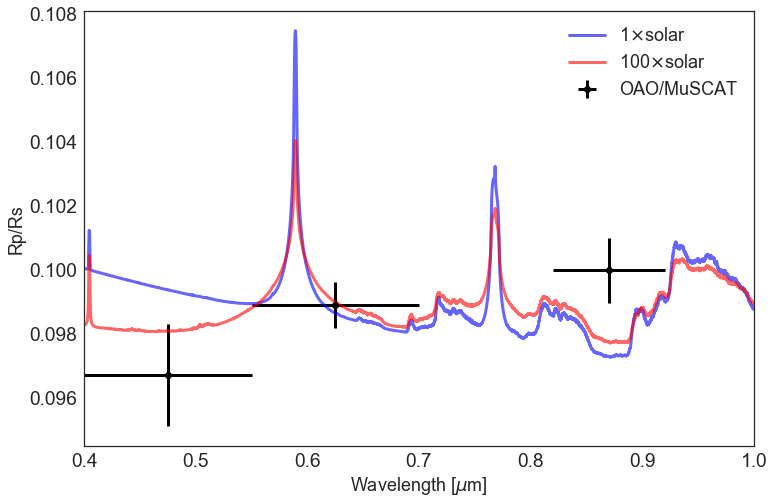
\includegraphics[width=12cm]{wasp21/atm_model.png}
\caption{Same as Fig~\ref{fig:atm_hatp12b} for WASP-21b but assuming $T_{eq}$ = 1340$\pm$32 K. The values of $\chi^2$ / d.o.f. are 3.2 and 2.4 for 1 $\times$ Solar and 100 $\times$ Solar atmospheres, respectively, implying that the data cannot be explained by either model.}
\label{fig:atm_wasp21b}
\end{figure}


\begin{comment}
The calculation is done based on the method described in Fukui et al. (2014), but in this case line absorption of H2S, OCS, O2, TiO, and VO are taken into account in addition to those treated in Fukui et al. (2014) (H2, H2O, CH4, CO, CO2, NH3, N2, Na, and K). 

Further, the absorption cross sections for these species are calculated on a wavelength-by-wavelength basis with a step size given by dividing the wavelength range from 0.3 to 1.0 μm by ∼2.5e5 in log scale without taking the geometric mean for a certain range of wavelengths as done in Fukui et al. (2014). An initial model spectrum is calculated by assuming that R0, the planetocentric distance at which the atmospheric pressure is 10
bar, is equal to 1.219 RJup (Southworth 2012).

Again, the observed Rp/Rs variations of this planet are too low with respect to the
observational uncertainties. 
\end{comment}